\documentclass{beamer}
%
% Choose how your presentation looks.
%
% For more themes, color themes and font themes, see:
% http://deic.uab.es/~iblanes/beamer_gallery/index_by_theme.html
%
\mode<presentation>
{
  \usetheme{Madrid}      % or try Darmstadt, Madrid, Warsaw, ...
  \usecolortheme{beaver} % or try albatross, beaver, crane, ...
  \usefonttheme{serif}  % or try serif, structurebold, ...
  \setbeamertemplate{navigation symbols}{}
  \setbeamertemplate{caption}[numbered]
} 

\usepackage{hyperref}
\usepackage[english]{babel}
\usepackage[utf8x]{inputenc}
\usepackage{pdfpages}
\usepackage{framed, color}
\definecolor{shadecolor}{rgb}{1,0.8,0.3}
\usepackage{color}
 
\definecolor{codegreen}{rgb}{0,0.6,0}
\definecolor{codegray}{rgb}{0.5,0.5,0.5}
\definecolor{codepurple}{rgb}{0.58,0,0.82}
\definecolor{backcolour}{rgb}{0.95,0.95,0.92}
\definecolor{pblue}{rgb}{0.13,0.13,1}
\definecolor{pgreen}{rgb}{0,0.5,0}
\definecolor{pred}{rgb}{0.9,0,0}
\definecolor{pgrey}{rgb}{0.46,0.45,0.48}
 
\usepackage{listings}
\lstset{language=Python,
  showspaces=false,
  showtabs=false,
  breaklines=true,
  showstringspaces=false,
  breakatwhitespace=true,
  commentstyle=\color{pgreen},
  keywordstyle=\color{pblue},
  stringstyle=\color{pred},
  basicstyle=\ttfamily,
  frame=lrbt,xleftmargin=\fboxsep,xrightmargin=-\fboxsep
}

\title[Ragazze Digitali 2019]{Ragazze Digitali A.A. 2018/2019}
\author{E. Salvucci - S. Gattucci - C. Varini}
\date{}

\AtBeginSection[]
{
  \begin{frame}<beamer>
    \frametitle{Outline}
    \tableofcontents[currentsection,currentsubsection]
  \end{frame}
}

\begin{document}

\setbeamertemplate{background}
{
\includegraphics[width=\paperwidth,height=\paperheight]{images/ragazze_digitali.jpg}}
\begin{frame}
\end{frame}

\setbeamertemplate{background}
% Python

\begin{frame}{Cosa faremo oggi}
    \vspace{0.8cm}
      Costruiremo un semplice gioco che chiameremo \textbf{Guess the number}. \newline
      Il computer penserà un numero da 1 a 20 e ci darà sei possibilità avvertendoci, per ognuna di esse, se il numero da noi tentato è più grande o più piccolo di quello che ha pensato.
\end{frame}

\begin{frame}{Guess the number}
    \texttt{Hello! What is your name?\newline
        Sofia\newline
        Well, Sofia, I am thinking of a number between 1 and 20.\newline
        Take a guess.\newline
        10\newline
        Your guess is too high.\newline
        Take a guess.\newline
        2\newline
        Your guess is too low.\newline
        Take a guess.\newline
        4\newline
        Good job, Sofia! You guessed my number in 3 guesses!
    }
\end{frame}

\begin{frame}[fragile]
\frametitle{Guess the number}
\begin{block}{Per iniziare}
	\begin{itemize}
		\item Apriamo Spyder, l'IDE che useremo per programmare in Python
		\item Troviamo già un file vuoto che ci aspetta..
		\item ..Salviamo il file  tramite \textbf{File} $\rhd$ \textbf{Save as}
		\item Rinominiamo il file \textit{guess.py}, selezioniamo la vostra cartella personale come cartella di destinazione e iniziamo a riemprlo di codice!
	\end{itemize}
\end{block}
    
\end{frame}
\setbeamertemplate{background}{}

\section{Moduli, import e funzione per generare numeri casuali}

\begin{frame}[fragile]
\frametitle{guess.py}
    \begin{lstlisting}
# This is a Guess the Number game
import random
guessesTaken = 0
print('Hello! What is your name?')
myName = input()
number = random.randint(1, 20)
    \end{lstlisting}
\end{frame}

\begin{frame}{Moduli, import e funzione per generare numeri casuali}
    \begin{block}{Istruzione di \texttt{import} e funzione \texttt{randint()}}
        \begin{itemize}
            \item Il comando \textbf{import} serve per importare un \textit{modulo}, ovvero un programma separato nel quale sono presenti altre funzioni
            \item Importiamo il modulo \textit{random} dal quale chiamiamo la funzione \texttt{randint()} che ci permette di generare un numero casuale all'interno del range formato dai due numeri passati in input dalla funzione. Salviamo questo numero nella variabile \textbf{\textrm{number}}
            \item Catturiamo l'input dell'utente tramite la funzione \texttt{input()} e mettiamolo nella variabile \textbf{\texttt{myname}}
        \end{itemize}
        
    \end{block}
\end{frame}

\begin{frame}{Moduli, import e funzione per generare numeri casuali}
    \begin{block}{Ora prova tu!}
        \begin{itemize}
            \item Spostati nella shell di Python
            \item Importa il modulo \texttt{random} tramite il comando \texttt{import random} e premi invio
            \item Invoca la funzione \texttt{randint()} tramite il comando \texttt{random.randint()} inserendo come parametri della funzione il range che vuoi tu!
        \end{itemize}
        
    \end{block}
\end{frame}

\section{Istruzioni di controllo di flusso e organizzazione in blocchi}

\begin{frame}[fragile]
\frametitle{guess.py}
\begin{lstlisting}
print('Well, ' + myName + ', I am thinking of a number between 1 and 20.')
for guessesTaken in range(6):
    print('Take a guess.')
    guess = input()
    guess = int(guess)
\end{lstlisting}
\end{frame}

\begin{frame}[fragile]
\frametitle{Istruzioni di controllo di flusso e organizzazione in blocchi}
    \begin{block}{Blocchi}
    \begin{itemize}
        \item Il codice può essere organizzato in \textit{blocchi}, ovvero delle linee di codice che hanno lo stesso numero di spazi prima dell'inizio
    \end{itemize}
        Riprendiamo il codice che abbiamo appena visto:
\begin{lstlisting}
for guessesTaken in range(6):
****print('Take a guess.')
****guess=input()
****guess=int(guess)
\end{lstlisting}
	\begin{itemize}
	\item Consideriamo ogni * come uno spazio, che chiameremo \textit{indentazione}.
	\end{itemize}
    \end{block}
\end{frame}

\begin{frame}[fragile]
\frametitle{Istruzioni di controllo di flusso e organizzazione in blocchi}
    \begin{block}{Blocchi}
    \begin{itemize}
        \item Ogni riga che è indentata con lo stesso numero di spazi, fa parte di un \textbf{blocco}.
        \item Nel nostro esempio, le istruzioni che sono indentate con 4 spazi (*) fanno tutte parte del blocco che parte dal comando \texttt{for}
        \item Il comando \texttt{for} segna l'inizio di un \textbf{loop} o \textbf{ciclo}
    \end{itemize}
    \end{block}
\end{frame}

\begin{frame}[fragile]
\frametitle{Istruzioni di controllo di flusso e organizzazione in blocchi}
    \begin{block}{For statement}
    \begin{itemize}
        \item Quando il compilatore incontra il comando \texttt{for}, entra nel blocco che segue il comando, esegue tutte le istruzioni del blocco e riparte dall'inizio del blocco.
        \item Questo loop viene eseguito tante volte quanto il numero passato alla funzione \texttt{range()}
        \item Vediamo un esempio
    \end{itemize}
    \end{block}
\end{frame}

\begin{frame}[fragile]
\frametitle{Istruzioni di controllo di flusso e organizzazione in blocchi}
\begin{block}{Ora prova tu!}
	Ora proviamo a copiare questo codice nella console di Python per vedere cosa succcede!
\end{block}
\begin{lstlisting}
for j in range(4):
    print('Hello! The variable j is set to', j)
\end{lstlisting}
    
\end{frame}

\section{Conversione di valori e Boolean data type}

\begin{frame}[fragile]
\frametitle{Conversione di valori e Boolean data type}
	\begin{block}{Conversione di valori o \textbf{casting}}
	\begin{itemize}
		\item La funzione \texttt{int()} restituisce il valore passato in input come un \texttt{integer}, un valore intero.
		\item Vediamo qualche esempio per capire
	\end{itemize}
	\end{block}
	\begin{lstlisting}
>>> int('42')
>>> 3 + int('2')
>>> int('forty-two')
	\end{lstlisting}
Copiamo ciascuna riga premendo subito invio sulla console di Python, e osserviamo cosa succede per ognuna delle 3 istruzioni

\end{frame}

\begin{frame}[fragile]
\frametitle{Conversione di valori e Boolean data type}
\begin{block}{Conversione di valori o \textbf{casting}}
	\begin{itemize}
		\item Come abbiamo notato, la funzione \texttt{int()} accetta come argomenti anche delle stringhe, purchè esse contengano solo numeri
		\item Oltre alla funzione di \texttt{int()}, le funzioni \textbf{\texttt{float()}} e \textbf{\texttt{str()}} agiscono nello stesso modo, convertendo l'argomento in valori \textbf{float} e \textbf{string} rispettivamente.
	\end{itemize}
\end{block}
\begin{lstlisting}
>>> float('42')
>>> float(96)
>>> str(58)
>>> str(58.36)
\end{lstlisting}
Copiamo ciascuna riga premendo subito invio sulla console di Python, e osserviamo cosa succede per ognuna delle istruzioni
\end{frame}

\begin{frame}[fragile]
\frametitle{Conversione di valori e Boolean data type}
\begin{block}{Boolean data type}
	\begin{itemize}
		\item Abbiamo visto in precedenza i "data type" che ogni valore può assumere, tra cui \textit{integer, float e string}.
		\item Il data type Boolean, \textbf{\textit{bools}} per gli amici, ha due valori: \texttt{True} o \texttt{False}
	\end{itemize}
\end{block}
\begin{lstlisting}
>>> var = True
>>> var
>>> var = False
>>> var
\end{lstlisting}
Copiamo ciascuna riga premendo subito invio sulla console di Python, e osserviamo cosa succede per ognuna delle istruzioni
\end{frame}

\section{Operatori di comparazione e if statement}

\begin{frame}[fragile]
\frametitle{guess.py}
	\begin{lstlisting}
****if guess < number:
********print('Your guess is too low.')
****if guess > number:
********print('Your guess is too high.')
****if guess == number:
********break
	\end{lstlisting}
\end{frame}

\begin{frame}[fragile]
\frametitle{Operatori di comparazione e if statement}
\begin{block}{Cosa vuol dire?}
	\begin{itemize}
		\item Le tre istruzioni \texttt{if} sono simili tra loro, e ciascuna di esse costituisce un \textbf{sotto-blocco} del blocco \texttt{for}
		\item \textbf{RICORDA!} \texttt{guess} e \texttt{number} sono due variabili che contengono entrambe un numero!
		\item L'istruzione \texttt{if}, \textbf{se} in italiano, indica una condizione per cui:\newline - \textbf{se è vera} viene eseguito il codice all'interno del sotto-blocco\newline - \textbf{altrimenti} viene eseguita quella successiva, SENZA eseguire l'istruzione all'interno.
		\item Vediamo di capire meglio con un esempio
	\end{itemize}
\end{block}
\end{frame}

\begin{frame}[fragile]
\frametitle{Operatori di comparazione e if statement - Esempio}
		\begin{columns}[T]
			\begin{column}[T]{0.5\textwidth}
				\begin{figure}[t]
					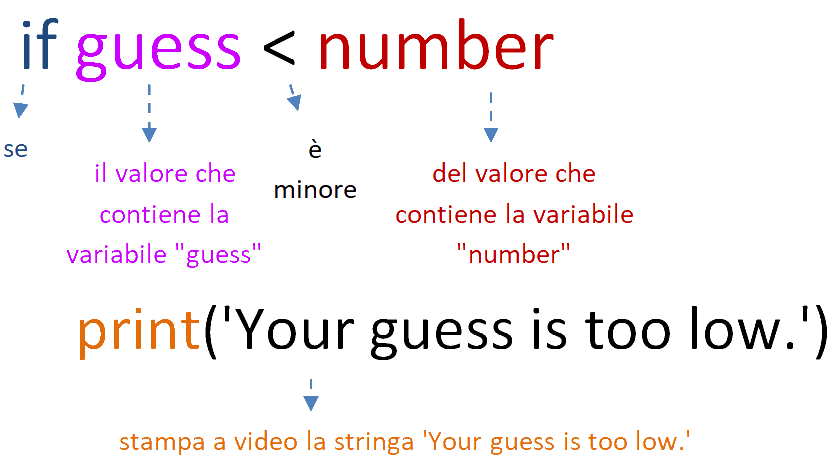
\includegraphics[height=3.7cm, width=\textwidth]{images/if.png}
				\end{figure}
			\end{column}
			\begin{column}[T]{0.5\textwidth}
				\begin{figure}[t]
					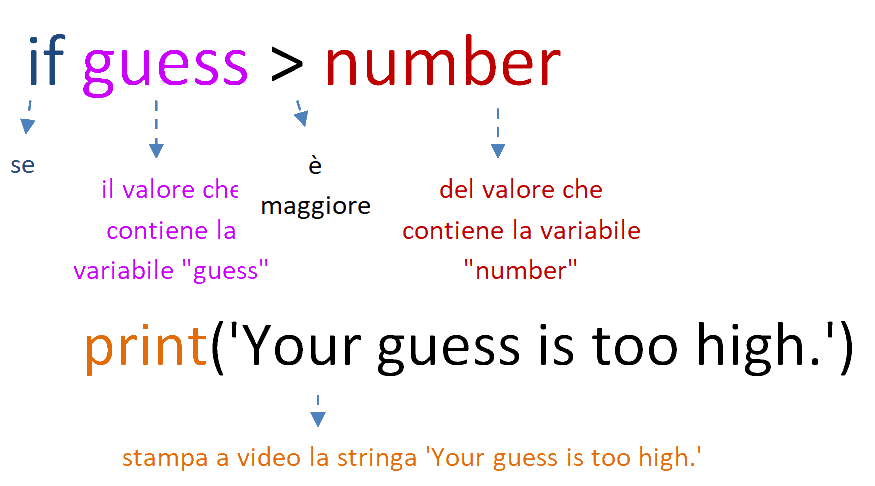
\includegraphics[height=3.7cm, width=\textwidth]{images/if2.png}
				\end{figure}
			\end{column}
		\end{columns}
	\begin{figure}
		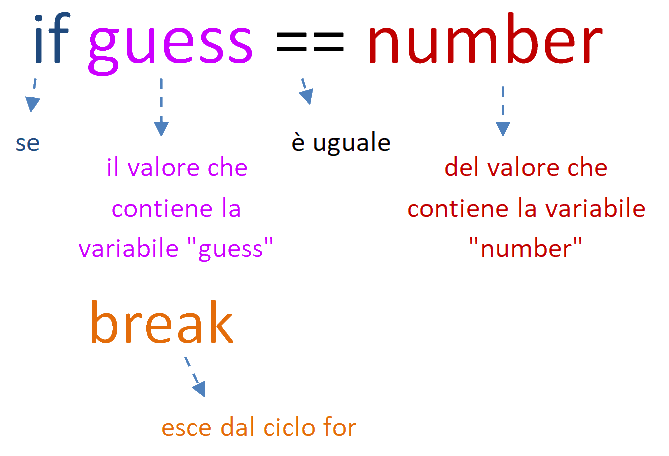
\includegraphics[height=3.7cm, width=0.5\textwidth]{images/if3.png}
	\end{figure}
\end{frame}

\begin{frame}[fragile]
\frametitle{Operatori di comparazione e if statement}
\begin{block}{Operatori di comparazione}
	\begin{itemize}
		\item Il comando \texttt{break} permette di interrompere l'esecuzione del ciclo \texttt{for} in anticipo, prima della sua fine naturale
		\item Abbiamo visto alcuni operatori di comparazione, vediamo ora i principali:
	\end{itemize}
\end{block}
\begin{center}
	\begin{tabular}{ c  c }
		\hline
		Operatore & Significato \\ 
		\hline
		$<$ & minore di \\  
		$>$ & maggiore di \\
		$<$= & minore uguale di \\  
		$>$= & maggiore uguale di \\
		== & uguale \\  
		$!$= & diverso 
	\end{tabular}
\end{center}
\end{frame}

\section{Ultime righe di codice}

\begin{frame}[fragile]
\frametitle{guess.py}
	\begin{lstlisting}
if guess == number:
    guessesTaken = str(guessesTaken + 1)
	print('Good job, ' + myName + '! You guessed my number in ' +
	guessesTaken + ' guesses!')
	
if guess != number:
	number = str(number)
	print("That\'s too bad. The number I was thinking of was " + number + ".")
	\end{lstlisting}
\end{frame}

\begin{frame}[fragile]
\frametitle{Ultime righe di codice}
	\begin{block}{Carattere di escape}
	\begin{itemize}
		\item C'è un'altra cosa strana in una delle due \texttt{print()}... A cosa serve quel \textbackslash prima dell'apice tra \textit{That} e \textit{s}?
		\item Viene usato, all'interno di stringhe, come \textbf{carattere di escape}
		\item Cos'è un carattere di escape? Serve per poter stampare i caratteri speciali che hanno già un loro significato, come l'apice ('), che viene interpretato come inizio stringa
		\item Vediamo ora cosa può permettere di stampare questo carattere di escape:
	\end{itemize}
\end{block}
\begin{center}
\begin{tabular}{ c  c }
	\hline
	Carattere di escape & Cosa viene stampato \\ 
	\hline
	\textbackslash \textbackslash & Backslash (\textbackslash)  \\
	\textbackslash ' & Apice(') \\
	\textbackslash " & Doppie virgolette (")\\  
	\textbackslash n & Andata a capo\\
	\textbackslash t & Tabulazione 
\end{tabular}
\end{center}
\end{frame}


\begin{frame}

\begin{center}
	\bigskip
	Materiale rilasciato con licenza
	
	\textbf{\href{http://creativecommons.org/licenses/by-sa/4.0/}{Creative Commons - Attributions, Share-alike 4.0}}
	
	\medskip
	
\includegraphics[height=0.8cm]{images/cc.jpeg}
\end{center}

\end{frame}	
\end{document}
